\chapter{Data acquisition software}

\epigraph{Before software can be reusable \\it first has to be usable.}{Ralph Johnson}

Data acquisition is a critical component of all particle physics experiments across all stages of technological readiness, from the very beginning of hardware testing in tabletop experiments to full-scale international experiments like the Large Hadron Collider. 

In the modern era of particle physics, the interplay of hardware and software at minscule timescales drives everything, and almost all results are highly dependent upon the speed and efficiency of the electronics and computer systems that extract data from the detectors. A massive quantity of work goes into creating, testing and optimising the systems that will acquire, process, sort and transport data before it is ever seen by the physicist operating the experiment.

Of particular interest in this thesis is the data acquisition software during the development phase, where individual detector subcomponents are undergoing prototyping and testing. These development and iteration cycles are tied closely to testbeam facillities such as the Super Proton Synchrotron (SPS) at CERN and the DESY II synchrotron at DESY. At this point in the development cycle, the detectors are beginning to take shape and this is where data acquisition (or DAQ) becomes an important consideration. 

In addition to this, the data acquisition solutions used during the testbeam phase of detector development is likely to inform the final data acquisition solution, either directly by evolving into the final software, or indirectly by identifying and evaluating the particular features or challenges of the subdetector components that the software must take into account or accommodate.

During this stage, each individual detector component -- such as a vertex tracker or hadronic calorimeter -- will be developed by small teams, and the natural tendency is for each of these groups to set their own standards and develop their own tools, prioritising the features that are important to their specific case. However, in the past this approach has generated a variety of \textit{ad hoc} solutions for testbeam software, many of which cannot be applied outside of their original scope. The also results in wasted effort and time, as different teams implement the same solutions anew for each subdetector.

One of the aims of the AIDA-2020 project is to improve this situation by developing generic and reusable software tools for testbeams and particle physics experiments.

\subsubsection{The AIDA-2020 project}
The AIDA-2020 project is an EU-funded research programme for developing infrastructure and technologies for particle physics detector development and testing, comprising 24 member countries and lead by CERN.

The overarching goal of the project is to develop common infrastructures and tools for physics testbeams, and software is one such important tool. By creating a suite of tools that are designed with a variety of uses in mind, the amount of effort and development time necessary to plan and implement data acquisition and monitoring setups can be significantly reduced or eliminated, speeding up the planning and deployment of physics testbeams. This allows more science to be done faster. The two tools within AIDA-2020 that facillitate this are EUDAQ and DQM4hep, discussed in more detail below.

\section{EUDAQ}
[...]

\section{DQM4hep}
Data Quality Monitoring for High-Energy Physics (abbreviated DQM4hep) is an online monitoring and data quality monitoring framework developed for physics testbeams for high-energy and particle physics. It is designed to be able to fulfil the requirements of monitoring for physics testbeams in a generic way. The structure of the program allows for independent components of the framework to be used, not used, or exchanged, by isolating each function of the program into specific and independent processes. The components that are specific to particular users -- the file readers, event streamers, and analysis and standalone modules -- are written in standard C++ code, meaning they are capable of performing any data unpacking, processing or analysis that is necessary. The framework then handles packaging this information in a useful way and networking to transmit it to where it is needed, meaning that the user does not have to worry about the mechanics of data storage, serialisation or transmission. It also means that the framework does not need special rules for handling particular datatypes, allowing it to handle \emph{anything} that can be packed into, decoded from, and accessed by normal C++ methods. This results in a framework that is able to deal with any kind of data, including user-defined data types, making it more flexible, portable and easily reusable.

\subsection{Prerequisites and dependencies}

DQM4hep is a C++ application, written in the C++11 standard, that can run on any Linux distribution. The only requirements for installation are a compiler compliant with the C++11 standard, cmake 3.4 or higher, and ROOT 6. All other prerequisites or dependencies are downloaded and compiled by the framework's installer. 

[...]

\subsection{Programming paradigms and structure}

The two core principles for DQM4hep are genericity and modularity. The core of the system is based on a plugin system to allow shared libraries to be loaded and hook classes for further use. \cite{aida2020-milestone-dqm4hep}

[...]

\begin{figure}[h]
	\centering
	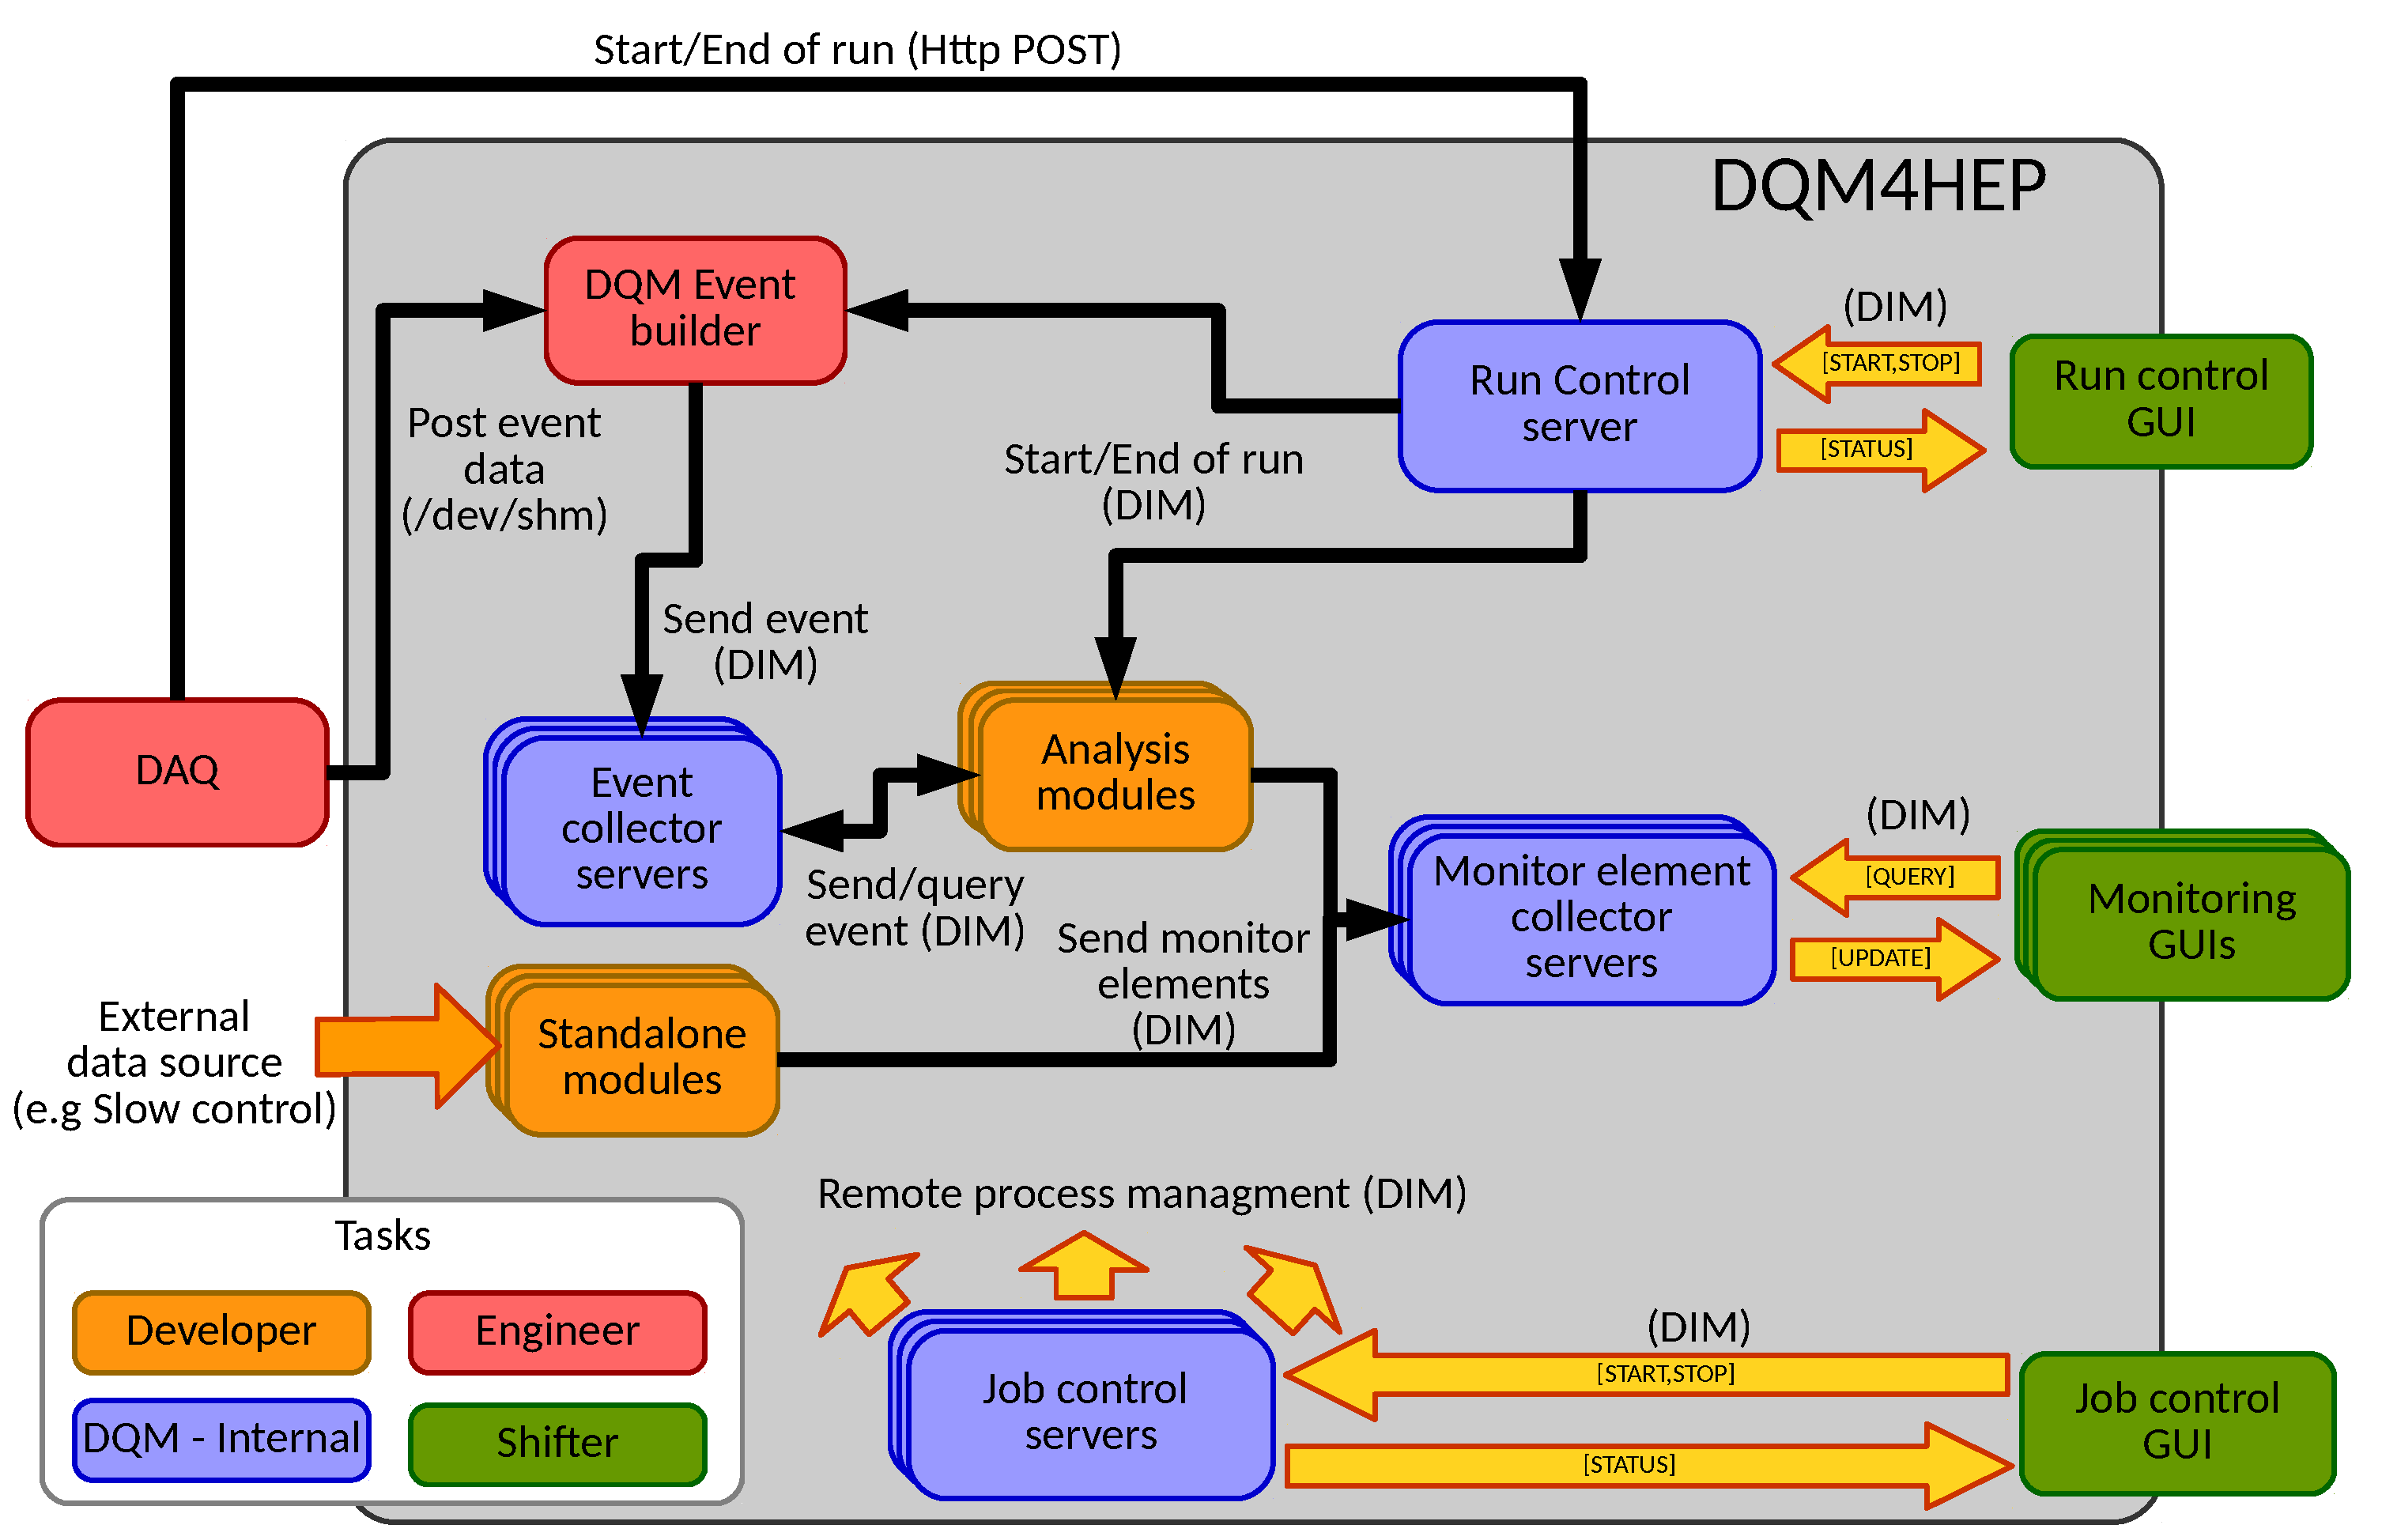
\includegraphics[width=0.95\textwidth]{../Pictures/GlobalArchitectureDiagram.pdf}
	\caption{The global online architecture of DQM4hep.}
	\label{figure:daq/dqm4hep/architecture}
\end{figure}

\subsection{Visualisation and graphical user interface}
As of writing, the graphic user interfaceand visualisation suite is still under active development.  Previous versions of DQM4hep have utilised the Qt framework for GUI and visualisation.

The decision to remove the Qt-based GUI from the framework was because of integration with ROOT -- running DQM4hep previously required an installation of ROOT that had the \texttt{--enable-Qt} flag, and the majority of ROOT installations in remotely-accsible file systems based at CERN and DESY (which are heavily used for analysis and testbeams) were not compiled with this flag. 

The removal of the Qt-based UI however allows for greater freedom with UI development. The intended goal is to have a browser-based UI, removing dependency on specific software frameworks, allowing it to function on any device. [...]

[...]

\subsection{Data quality testing}
One of the important areas of DQM4hep that was not yet completed was data quality monitoring, which is an array of tests or programs that assess the data being taken in real time to allow testbeam operators and shifters without detailed knowledge of the hardware, software, or physics to determine whether the device under test is performing as intended, and to quickly identify and address any errors or inconsistencies. Data quality monitoring (DQM) uses a variety of methods for measuring the `quality' or `goodness' of data, mainly relying upon statistical or comparative methods.

DQM4hep did not have any infrastructure to support data quality tests, but this was added during the core refactoring for the release version [?]. Once this was in place, a variety of data quality tests were developed and implemented, ranging from basic tests, such as comparing the mean of a data sample against predefined values of mean and standard deviation, to more complex tests, such as the Kolmogorov-Smirnov test, which is a comparison between a sample and a reference histogram.

% Here we should have figures demonstrating the qtests. Maybe one mean/stddev (if we can find visual information for this), and one comparison to reference, e.g. Kolmogorov.

[...]

\section{Adaptation to other detectors}

[...]

To utilise DQM4hep with any new detector, either two or three new plugins must be created depending on whether the detector is to be monitored online, offline, or both.

If the data is to be monitored offline, then a file reader plugin must be written. If the data is to be monitored online, then a streamer plugin must be written. Both of these plugins are similar in structure and differ only on where they get the data from -- a file reader loads a file from disk, whereas a streamer loads it from the data acquisition system. Once the information is accessible from the reader plugin, it packages the data into events, and emits them to the framework's network handling to be received by any other plugins that are listening for them. The incoming data can be of any type, since the methods for reading it are provided in the reader plugin itself. Previously, reader plugins have been created to read binary files, raw text files, SLCIO data files, and ROOT trees.

An analysis module is a type of plugin which takes data that is packaged into events by a reader plugin and performs some analysis on it. Each analysis module can only read events from one reader, but [...] 

Writing new readers and analysis modules is relatively simple, especially if the data has already been packaged into well-structured formats such as ROOT or SLCIO. [...]

% Place an example file reader here, well-commented?

\section{Integration with EUDAQ}
[...]

\section{Documentation and user guide}

One of the biggest hurdles to promoting a new framework is the lack of understanding of it's installation, deployment, and usage. Many research teams will continue to use their existing software solutions, which may be suboptimal or difficult to use, according to the principle of `better the devil you know than the devil you don't`. The first step to overcoming this is to produce clear, readable and complete documentation across the entire range of features the framework has.

[...]

Many particle physics software frameworks provide documentation in the form of Doxygen, a documentation generator tool. Doxygen is extremely useful, as the documentation for functions and objects is written within the code itself, ensuring that documentation is written as the code is written. Doxygen also automatically compiles a documentation guide using HTML, automatically listing the relationships between objects, structures, functions, etc. that can be compiled and viewed locally, or hosted on the internet as a reference.

One issue with Doxygen documentation is that is not holistic. Doxygen compiles documentation for individual structures of the program, not of the program as a whole. Doxygen is extremely useful for developers, as well as alread-experienced users. However it doesn't aid new users in learning to use   a piece of software, 

[...]

An important aspect with this holistic documentation was that it was to be very distinct from the developer documents (i.e. Doxygen). These were to be a set of guides and walkthroughs for common procedures, intended for \emph{users} of the framework with little to no interest in the mechanics of it.

[...]

\subsection{File reader plugins}
[...]

\subsection{File streamer plugins}
[...]

\subsection{Analysis and standalone modules}
[...]
